\section{Lezione 1}%
\label{sub:Lezione 1}

\subsection{Moto Browniano}%
Il conte Brown nel 1827 pensò di aver scoperto la vita osservando particelle di polline in acqua che si muovevano in modo casuale, ne concluse che le particelle fossero vive. Successivamente fu Einstein a dare una descrizione collisionale con i seguenti punti chiave:
\begin{itemize}
    \item Impatti frequenti.
    \item Descrizione probabilistica.
    \item Dinamica discreta (tempo discretizzato).
\end{itemize}
Mettiamoci in un sistema unidimensionale e ipotizziamo che il tempo caratteristico di impatto tra due palline sia $\tau$ e che $n(t)$ sia il numero delle palline.\\
Sempre per ipotesi per ogni pallina si ha la proprietà:
\[
    x(t=0) = x \implies  x(t=\tau) = x + \Delta
.\] 
Dove $\Delta$ varia da pallina a pallina, possiamo definire una distribuzione pari di questi $\Delta$: $f(\Delta)$
\[\begin{aligned}
    &\int f(\Delta) d\Delta = 1; \quad &f(\Delta) = f(-\Delta) 
.\end{aligned}\]
\paragraph{Primo esempio di equazione di Fokker-Plank}%
Possiamo trovare il numero $dn$ di palline che si muovono di una quantità $\xi$: $\Delta < \xi < \Delta  + d\Delta$.
\begin{figure}[H]
    \centering
    \incfig{1-brown}
    \caption{\scriptsize Particelle che si muovono di $\xi$, dove $\Delta$ è la variabile stocastica per le palline.}
    \label{fig:1-brown}
\end{figure}
\noindent
\[
    dn = n f(\Delta) d\Delta
.\] 
La probabilità che una pallina si trovi nel punto $x$ al tempo $t+\tau$ per $dx$ è:
\begin{greenbox}{Equazione di Chapman-Kolmogorov}
 \begin{equation}
    P(x,t+\tau) dx = dx \int P(x-\Delta,t) f(\Delta) d\Delta \label{eq:CK_1}
\end{equation}
\end{greenbox}
\noindent
L'equazione rappresenta il fatto che il processo in question è markoviano. Se così non fosse avremmo dovuto mettere a destra più di un tempo (anticipazione di argomento del corso).\\
Espandendo in serie (di Kramers-Moyal) le probabilità:
\[\begin{aligned}
    &P(x, t+\tau) = P(x, t) + \frac{\partial P}{\partial t} \tau  \\
    & P(x-\Delta,t) = P(x,t) - \frac{\partial P}{\partial x} \Delta  + \frac{1}{2}\frac{\partial ^2 P}{\partial x^2} \Delta^2
.\end{aligned}\]
Si ottiene reinserendo nella \ref{eq:CK_1}:
\begin{redbox}{Equazione del tipo di Fokker-Plank}
     \begin{equation}
	\frac{\partial P}{\partial t} = D \frac{\partial ^2P}{\partial x^2} \label{eq:FP_1}
    \end{equation}
Nella quale $D$ vale:
\[
    D = \frac{1}{2\tau}\left<\Delta^2\right>
.\]    
\end{redbox}

\noindent
Integrando la \ref{eq:FP_1} si ottiene, con le condizioni iniziali: $P(x,t=0) = \delta(x)$
\[
    P(x,t) = \frac{n}{\sqrt{4\pi Dt}}\exp\left(-\frac{x^2}{4Dt}\right)   
.\] 
\subsection{Dinamica mesoscopica: Langevin}%
Possiamo scrivere una equazione del moto per le palline tenendo di conto di:
\begin{itemize}
    \item Attrito: $-6\pi\eta d \dot{x}$ (Approccio alla Stokes) 
    \item Impatti random tra le altre particelle: $\xi$.
\end{itemize}
\begin{equation}
    m\ddot{x} = -6\pi\eta d \dot{x} + \xi
\end{equation}
Che è un primo esempio di equazione differenziale stocastica.\\
Se moltiplichiamo a destra e sinistra per $x$  possiamo riscriverla nel seguente modo:
\[
    \frac{1}{2}m\frac{\text{d} ^2}{\text{d} t^2}\left(x^2\right) - m\dot{x}^2 = -3\pi\eta d \frac{\text{d} }{\text{d} t}\left(x^2\right) + \xi x
.\] 
Possiamo mediare su tutte le possibili realizzazioni della $\xi$:
\[
    \frac{m}{2}\frac{\text{d} ^2}{\text{d} t^2} \left<x^2\right>-kT = -3\pi\eta d \frac{\text{d} }{\text{d} t} \left<x^2\right>
.\] 
Si risolve con metodi noti:
\[
    \frac{\text{d} }{\text{d} t} \left<x^2\right>=\frac{kT}{3\pi\eta d}+ C\exp\left(\frac{-6\pi\eta dt}{m}\right)
.\] 
Possiamo buttare il secondo termine ottenendo:
\begin{redbox}{Equazione di diffusione}
    \begin{equation}
       \left<x^2\right>_t-\left<x^2\right>_0 = \frac{kT}{3\pi\eta d}\cdot t
    \end{equation}
\end{redbox}
Andando a vedere l'equazione di Fokker-Plank vista sopra si scopre che c'è una relazione tra $D$  ed i coefficienti di questa equazione:
\begin{bluebox}{Coefficiente di Einstein}
    \[
        D = \frac{kT}{6\pi\eta d}
    .\] 
    Detto anche coefficiente di diffusione.
\end{bluebox}
\subsection{Nascita-Morte: Master equation}%
Ipotizziamo di avere due specie di animali:
\begin{itemize}
    \item Conigli: $x$ 
    \item Volpi: $y$ 
\end{itemize}
Tali animali possono essere modellizzati con il seguente modello di nascite/morti:
\begin{greenbox}{Sistema di Lotka-Volterra}
 \[
    \begin{cases}
	&x+\text{food}\to 2x\\
	&x+y\to 2y\\
	&y\to \text{death}
    \end{cases}
.\]    
\end{greenbox}
\noindent
Possiamo tradurre questo sistema con due equazioni differenziali (ad intuito):
\[
    \begin{cases}
	&\frac{\text{d} x}{\text{d} t} =k_1xc-k_2xy\\
	&\frac{\text{d} y}{\text{d} t} = k_2xy-k_3y
    \end{cases}
.\] 
\begin{figure}[H]
    \centering
    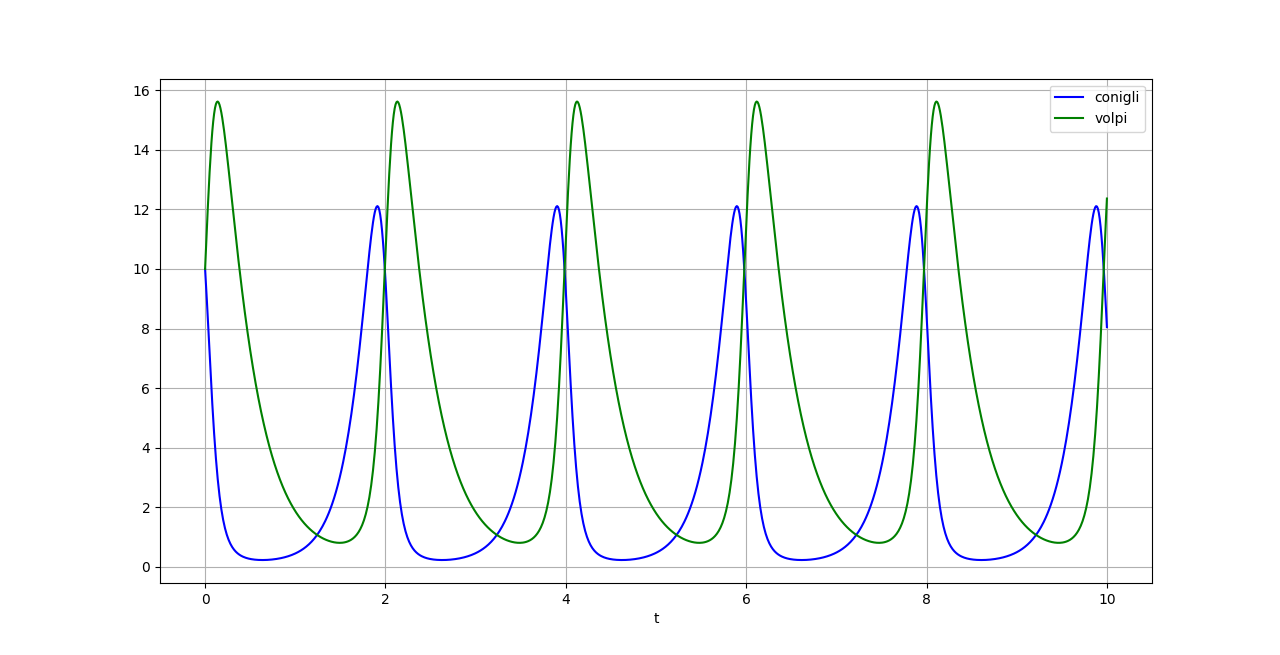
\includegraphics[width=0.4\textwidth]{figures/Volpi-Conigli.png}
    \caption{\scriptsize Andamento delle soluzioni}
    \label{fig:conigli}
\end{figure}
\begin{lstlisting}[language=Python]
from scipy.integrate import odeint
import matplotlib.pyplot as plt
import numpy as np
def func(y,t, c, k1, k2, k3):
    r,s = y 
    drds = [k1*c*r-k2*r*s, k2*r*s - k3*s]
    return drds
k1 = 1
k2 = 5
k3 = 1
c = 3
t0 = [10, 10]
t = np.linspace(0,10,1000)
sol = odeint(func, t0, t, args=(k1, k2, k3, c))
plt.plot(t, sol[:, 0], 'b', label='conigli')
plt.plot(t, sol[:, 1], 'g', label='volpi')
plt.legend(loc='best')
plt.xlabel('t')
plt.grid()
plt.show()
\end{lstlisting}
Come possiamo tener di conto delle fluttuazioni presenti in natura?\\
In realtà dovremmo utilizzare un modello discreto, quindi possiamo migliorare il metodo visto in precedenza. Prendiamo la probabilità di avere $(x,y)$ (lepri, volpi) al tempo $t$: $P(x,y,t)$ (dove adesso $x,y$ sono discreti). Valgono le seguenti uguaglianze per un certo tempo $\Delta t$:
\[\begin{aligned}
    &P_r(x\to x+1, y) \Delta t = k_1 c x \Delta t\\
    &P_r(x\to x-1, y \to y+1) \Delta t  = k_2xy\Delta t\\
    &P_r(x\to x,y\to y-1) \Delta t = k_3 y \Delta t\\
    &P(x\to x,y\to y) \Delta t = \Delta t \left[  1 - \left(k_1cx+ k_2xy + k_3 y\right)\right]
.\end{aligned}\]
Dove $P_r$ è la probabilità di fare la transizione (indipendente da $t$ per ipotesi).
Possiamo trovare l'evoluzione temporale come:
\begin{redbox}{Esempio di Master Equation}
    \begin{equation}
        \begin{aligned}
	    &\frac{P(x,y,t+\Delta  t) - P(x,y,t)}{\Delta  t}  =\\
	    & \quad P_r(x-1\to x, y) \cdot P(x-1,y,t) +\\
	    & \quad P_r(x+1\to x, y-1\to y) \cdot P(x+1,y,t) + \\
	    & \quad P(x\to x, y+1\to y) P(x,y+1,t) + \\
	    & \quad \left[P_r(x\to x, y\to y) - 1\right]\cdot P(x,y,t) 
        \end{aligned}
    \end{equation}
\end{redbox}
